\section[CMP Method]{The CMP Method}

\begin{frame}{Bayesian Calibration of Mis-Specified Models}
    \begin{center}
        \Large \textbf{The Complete Maximum a Posteriori (CMP) Method} \\[0.5cm]
        \normalsize How can we overcome the curse of dimensionality while preserving the rigor of a Full Bayesian analysis?
    \end{center}
\end{frame}

\begin{frame}{The Full Bayesian (FB) Formulation}
    In a Full Bayesian approach, we try to estimate the physical parameters $\btheta$ and the model error hyperparameters $\bpsi$ at the same time:
    \begin{equation*}
        \p{\btheta, \bpsi \mid \data} \propto \likelihood{\data \mid \btheta, \bpsi} \prior{\btheta} \prior{\bpsi}
    \end{equation*}
    To find what we actually care about (the physical parameters), we have to integrate out the hyperparameters:
    \begin{equation*}
        \p{\btheta \mid \data} = \intpsi{\p{\btheta, \bpsi \mid \data}}
    \end{equation*}
    
    \vspace{0.3cm}
    \textbf{The catch?} This integration is computationally prohibitive in high dimensions. It simply takes too long.
\end{frame}

\begin{frame}{The Modular Approach (KOH) and its Limitations}
    To avoid this bottleneck, the classic Kennedy and O'Hagan (KOH) approach suggests estimating the hyperparameters independently first:
    \begin{equation*}
        \psikoh = \argmax_{\bpsi} \intt{\p{\btheta, \bpsi \mid \data}}
    \end{equation*}
    Then, we just plug that estimate back in to find our parameters:
    \begin{equation*}
        \p{\btheta \mid \data, \psikoh} \propto \likelihood{\data \mid \btheta, \psikoh} \prior{\btheta}
    \end{equation*}
    
    \vspace{0.3cm}
    \textbf{The problem?} By completely ignoring the uncertainty in $\bpsi$, we end up with \textit{false certitude}—our parameter estimates look much more confident than they actually are, which can introduce dangerous bias.
\end{frame}

\begin{frame}{Introducing the Complete Maximum a Posteriori (CMP) Method}
    So, how do we fix this? Enter the Complete Maximum a Posteriori (CMP) Method.
    \vspace{0.3cm}
    
    The goal is straightforward: keep the computational efficiency of modular approaches, but perfectly match the exact Full Bayesian posterior. Instead of relying on a single, fixed $\psikoh$, we define a flexible functional mapping:
    \begin{equation*}
        \psimap = \argmax_{\bpsi \in \Psi} \p{\btheta, \bpsi \mid \data}
    \end{equation*}
    
    This couples $\bpsi$ back to $\btheta$, letting us evaluate the joint posterior along a parameter-dependent curve $\left(\btheta, \psimap\right)$.
\end{frame}

\begin{frame}{Functional Mapping: Decoupling with Coherence}
    If we break down the joint posterior using the marginal probability rule, we get:
    \begin{equation*}
        \p{\btheta, \bpsi \mid \data} = \p{\btheta \mid \data} \p{\bpsi \mid \btheta, \data}
    \end{equation*}
    
    \vspace{0.5cm}
    By looking at this, we realize that evaluating the conditional distribution $\p{\bpsi \mid \btheta, \data}$ right at its peak ($\psimap$) gives us a clever shortcut. It provides a direct pathway to marginalize the joint distribution without ever having to actually compute the difficult integral.
\end{frame}

\begin{frame}{Hessian-Based Correction Factor}
    Assuming the shape of the conditional distribution changes only by shifting and scaling:
    \begin{equation*}
        \bphi = \Stheta (\bpsi - \psimap)
    \end{equation*}
    We introduce a crucial Hessian-based correction factor $\detf{\Stheta}$ to the CMP posterior to keep everything mathematically sound:
    \begin{equation*}
        \p{\btheta \mid \data} \approx \p{\btheta, \psimap \mid \data} \dfrac{1}{\detf{\Stheta}}
    \end{equation*}
    
    \vspace{0.3cm}
    \begin{center}
        \begin{tikzpicture}[node distance=1.5cm, auto, thick, >={Stealth}]
            \node[draw, rounded corners, fill=blue!10] (map) {Compute $\psimap$};
            \node[draw, rounded corners, fill=red!10, right=of map] (hess) {Evaluate $\detf{\Stheta} \propto \sqrt{\detf{\hessian{\bpsi}}}$};
            \node[draw, rounded corners, fill=green!10, right=of hess] (post) {Corrected $\p{\btheta \mid \data}$};
            
            \draw[->] (map) -- (hess);
            \draw[->] (hess) -- (post);
        \end{tikzpicture}
    \end{center}
\end{frame}

\begin{frame}{Analytical Equivalence to Full Bayesian}
    Does this actually work? We start with a \textbf{Closed-Form Example: Well-Specified Model}.
    \vspace{0.3cm}
    
    Here, there is no structural model error, only experimental noise ($\sigma_e$).
    \begin{itemize}
        \item In this closed-form scenario, CMP perfectly matches the exact Full Bayesian marginal posterior.
        \item Traditional modular approaches suffer from \textbf{false certitude}, overemphasizing areas with small residuals and completely failing to capture the heavier tails of the true distribution.
        \item The Hessian correction factor $\detf{\Stheta}$ is what theoretically guarantees CMP's accuracy here.
    \end{itemize}
\end{frame}

\begin{frame}{Closed-Form Example: Mixture of Gaussians}
    What happens if the posterior is highly multimodal? We tested CMP on a theoretical Mixture of Gaussians.
    \vspace{0.3cm}
    
    \begin{columns}
        \begin{column}{0.5\textwidth}
            \centering
            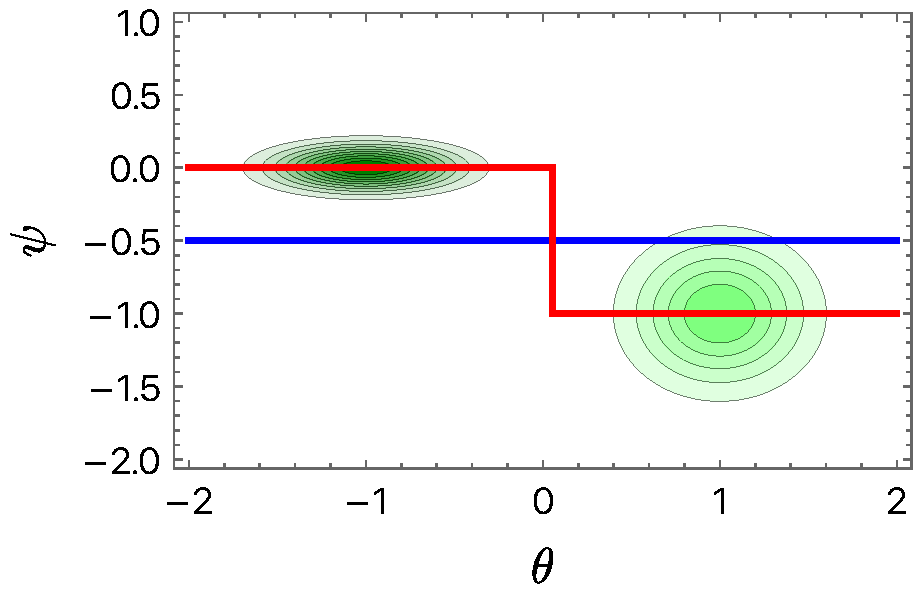
\includegraphics[width=0.9\textwidth,height=0.45\textheight,keepaspectratio]{../figures/cmp/fig_3.pdf}
            \\[0.1cm]
            \footnotesize Joint distribution with the $\psimap$ curve (red).
        \end{column}
        \begin{column}{0.5\textwidth}
            \centering
            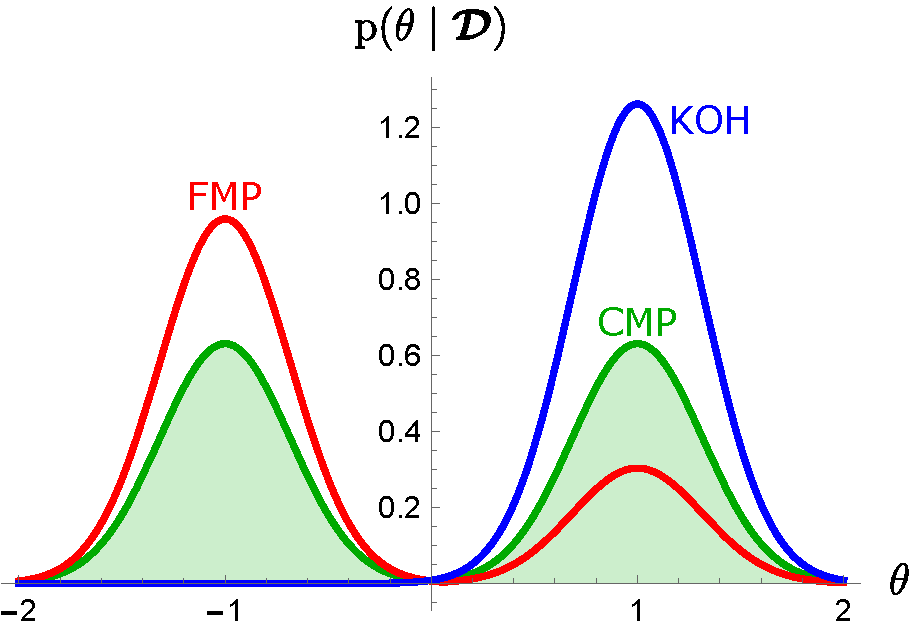
\includegraphics[width=0.9\textwidth,height=0.45\textheight,keepaspectratio]{../figures/cmp/fig_4.pdf}
            \\[0.1cm]
            \footnotesize CMP posterior matches exactly.
        \end{column}
    \end{columns}
    \vspace{0.3cm}
    CMP exactly recovers the modes and their true weights, whereas KOH collapses to a single mode.
\end{frame}

\begin{frame}{Numerical Example: Higher Dimensional Unimodal Distribution}
    We then tested CMP on a complex numerical problem with an inadequate forward model and a Gaussian Process model error term.
    
    \begin{columns}
        \begin{column}{0.5\textwidth}
            \centering
            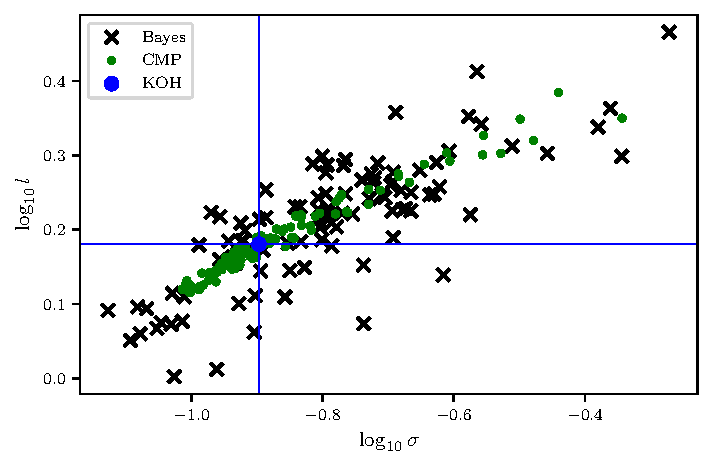
\includegraphics[width=\textwidth,height=0.5\textheight,keepaspectratio]{../figures/cmp/fig_9.pdf}
            \\[0.1cm]
            \footnotesize Joint plot of GP hyperparameters with $\psimap$.
        \end{column}
        \begin{column}{0.5\textwidth}
            \centering
            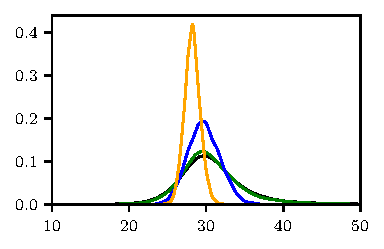
\includegraphics[width=\textwidth,height=0.5\textheight,keepaspectratio]{../figures/cmp/fig_8a.pdf}
            \\[0.1cm]
            \footnotesize Marginal posterior (CMP in green).
        \end{column}
    \end{columns}
    
    \vspace{0.3cm}
    Once again, CMP seamlessly captures the exact variance of the Full Bayesian method, avoiding the catastrophic overconfidence of KOH.
\end{frame}

\begin{frame}{Key Takeaway}
    \begin{block}{The Complete Maximum a Posteriori (CMP) Method}
        It successfully reduces a computationally expensive high-dimensional Full Bayesian problem into decoupled optimization steps. By using the Hessian correction, it explicitly prevents the False Certitude effect while maintaining scalability.
    \end{block}
\end{frame}

\section{Adaptive Sampling for CMP (AS-hGP)}

\begin{frame}{Accelerating CMP: The Computational Bottleneck}
    \begin{itemize}
        \item The CMP framework provides a robust posterior, but requires solving an optimization problem for the hyperparameters $\hat{\bpsi}_{\btheta}$ at each evaluation of $\btheta$.
        \item \textbf{Solution:} Replace the expensive mapping $\btheta \mapsto \hat{\bpsi}_{\btheta}$ with a surrogate model.
        \item \textbf{Hyperparameter Gaussian Processes (hGP):} Train a GP to predict $\hat{\bpsi}_{\btheta}$ across the parameter space.
        \item \textbf{Challenge:} Where to place the training points? We want to sample where the posterior is high, but the posterior is unknown a priori. Traditional one-shot sampling (e.g., LHS) is inefficient.
    \end{itemize}
\end{frame}

\begin{frame}{The AS-hGP Algorithm}
    AS-hGP iteratively builds the surrogate model by adaptively sampling from the posterior:
    \vspace{0.3cm}
    \begin{center}
    \begin{tikzpicture}[
        scale=0.8, transform shape,
        node distance=1.0cm and 1.5cm,
        block/.style={rectangle, draw=blue!80, thick, rounded corners, fill=blue!5, text width=4.5cm, text centered, minimum height=1.8cm, font=\small},
        arrow/.style={-{Stealth[scale=1.2]}, thick, draw=black!70},
        cond/.style={font=\footnotesize\itshape, fill=white, inner sep=2pt}
    ]

    % Nodes
    \node[block] (step1) {\textbf{Step 1: Build Surrogate}\\[1ex] $\tilde{\bpsi}(\btheta) \sim \mathcal{GP}$};
    \node[block, right=of step1] (step2) {\textbf{Step 2: Candidate Sampling}\\[1ex] $\btheta_c \sim \pi_{\text{avg}}(\btheta \mid \data)$};
    \node[block, below=of step2] (step3) {\textbf{Step 3: EVR Resampling}\\[1ex] $w_{\mathrm{res}}(\btheta) \propto \mathbb{V}_{\boldsymbol{\omega}} \left[ \phi(\btheta \mid \tilde{\bpsi}^{(\boldsymbol{\omega})})\right]$};
    \node[block, left=of step3] (step4) {\textbf{Step 4: Update}\\[1ex] $\boldsymbol{\Psi}^{(t+1)} = \boldsymbol{\Psi}^{(t)} \cup \{\text{new points}\}$};

    % Initialization and Exit
    \node[above=1cm of step1, align=center, font=\small] (init) {Initial Training Set $\boldsymbol{\Psi}^{(0)}$};
    \node[left=1.5cm of step4, align=center, font=\small] (end) {Final Surrogate\\ $\tilde{\boldsymbol{\psi}}^{(\star)}(\boldsymbol{\theta})$};

    % Arrows
    \draw[arrow] (init) -- (step1);
    \draw[arrow] (step1) -- (step2);
    \draw[arrow] (step2) -- (step3);
    \draw[arrow] (step3) -- (step4);
    \draw[arrow] (step4) -- node[right, cond] {not converged} (step1);
    \draw[arrow] (step4) -- node[above, cond] {converged} (end);

    \end{tikzpicture}
    \end{center}
\end{frame}

\begin{frame}{AS-hGP: Candidate Sampling}
    \begin{block}{Posterior-Informed Candidate Sampling}
        Candidate points are sampled from an averaged posterior over multiple GP realizations to prevent overfitting to the predictive mean.
    \end{block}
\end{frame}

\begin{frame}{AS-hGP: Variance-Based Weighted Resampling}
    \begin{block}{Variance-Based Weighted Resampling}
        Candidates are resampled using weights proportional to the variance of the potential:
        \begin{equation*}
            w_{\mathrm{res}}(\btheta_i) \propto \mathbb{V}_{\boldsymbol{\omega}} \left[ \phi(\btheta_i \mid \tilde{\bpsi}^{(\boldsymbol{\omega})}(\btheta_i))\right]
        \end{equation*}
        \begin{itemize}
            \item \textbf{Exploitation:} Candidates are already in high-probability regions.
            \item \textbf{Exploration:} Weights favor regions with high surrogate uncertainty.
            \item \textbf{Efficiency:} Rank-1 updates to the covariance inverse prevent selecting clustered points.
        \end{itemize}
    \end{block}
\end{frame}

\begin{frame}{Application: Design Under Uncertainty}
    \begin{itemize}
        \item We motivate AS-hGP using a \textbf{Design Under Uncertainty} problem.
        \item \textbf{Goal:} Predict the horizontal displacement of a planar frame.
        \item \textbf{Uncertainty:} The material (Young's modulus) is unknown and calibrated from a separate cantilever beam experiment. Unmodeled material nonlinearities act as model error.
    \end{itemize}
    \begin{center}
        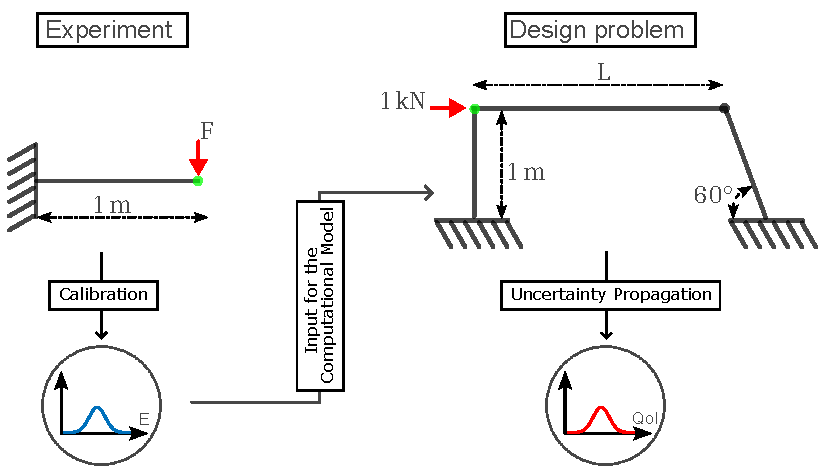
\includegraphics[width=0.9\textwidth,height=0.45\textheight,keepaspectratio]{../figures/surr/fig_4.pdf}
    \end{center}
\end{frame}

\begin{frame}{Results: Efficiency and Reliability}
    \begin{columns}
        \column{0.5\textwidth}
        \centering
        \textbf{Adaptive vs One-Shot Sampling}\\
        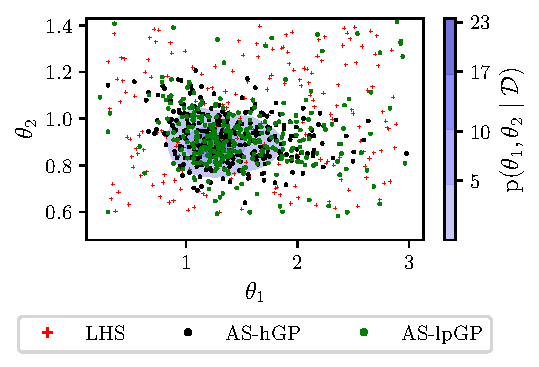
\includegraphics[width=\textwidth,height=0.6\textheight,keepaspectratio]{../figures/surr/fig_3.pdf}\\
        \footnotesize{AS-hGP concentrates training points around the true posterior (blue), unlike LHS (red).}
        
        \column{0.5\textwidth}
        \centering
        \textbf{Design Problem Prediction}\\
        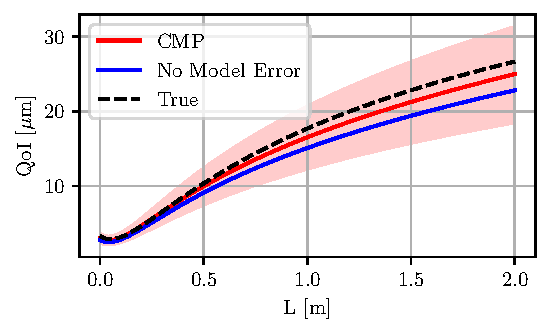
\includegraphics[width=\textwidth,height=0.6\textheight,keepaspectratio]{../figures/surr/fig_8.pdf}\\
        \footnotesize{Propagated AS-hGP posterior captures the true frame displacement reliably.}
    \end{columns}
\end{frame}

\section[Hypersonic Application]{Real-World Application: Hypersonic Flow Characterization}

\begin{frame}{VKI Plasmatron Experimental Setup}
    \begin{columns}
        \begin{column}{0.5\textwidth}
            \textbf{Our Goal}: Reconstruct catalytic efficiencies of reusable Thermal Protection Materials (TPMs) for hypersonic re-entry.
            
            \vspace{0.3cm}
            \begin{itemize}
                \item \textbf{Facility}: The VKI inductively-coupled-plasma wind tunnel.
                \item \textbf{Measurements}: We monitor the stagnation heat-flux ($q_w$) and stagnation pressure.
            \end{itemize}
        \end{column}
        \begin{column}{0.5\textwidth}
            \centering
            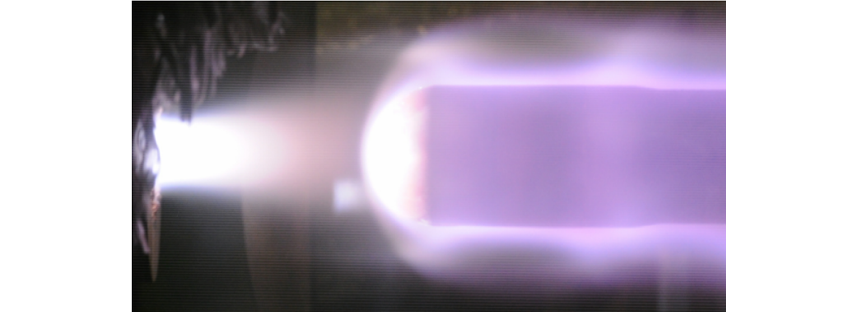
\includegraphics[width=\textwidth]{../figures/cfd/SupersonicJet.pdf}
            \\[0.2cm]
            \footnotesize Supersonic under-expanded air jet testing a TPM sample.
        \end{column}
    \end{columns}
\end{frame}

\begin{frame}{Formulating the Calibration Problem}
    Here is the catch: the total temperature $\mathrm{T}_0$ is \textit{unknown} and we can't measure it directly in the facility. 
    
    \vspace{0.3cm}
    So, we have to infer it alongside the catalytic efficiencies! Our calibration setup looks like this:
    \begin{equation*}
        \left.
        \begin{aligned}
            &q_\mathrm{w} = \tilde{q}_\mathrm{w}(\mathbf{p}; \gamma_{\mathrm{N}}, \mathrm{T}_0) + z_{q_\mathrm{w}} + \epsilon_{q_\mathrm{w}} \\
            &\mathrm{P}_\mathrm{w} = \hat{\mathrm{P}}_\mathrm{w}(\mathbf{p}; \gamma_{\mathrm{N}}, \mathrm{T}_0) + z_{\mathrm{P}_\mathrm{w}} + \epsilon_{\mathrm{P}_\mathrm{w}} \\
            &\dot{m} = \hat{m}(\mathbf{p}; \gamma_{\mathrm{N}}, \mathrm{T}_0) + z_{\dot{m}} + \epsilon_{\dot{m}} 
        \end{aligned}
        \right.
    \end{equation*}
    where $\mathbf{p}$ are our known pressure control variables.
\end{frame}

\begin{frame}{Two Types of Model Error}
    To rigorously test our framework, we deliberately introduce realistic model error by employing two different solvers:
    \vspace{0.3cm}
    \begin{columns}
        \begin{column}{0.5\textwidth}
            \begin{itemize}
                \item \textbf{Experimental Bias}: We introduce an artificial bias to the heat-flux measurements to emulate un-modeled facility effects.
                \item \textbf{Model Discrepancy}: We compare predictions from a high-fidelity 3D \texttt{US3D} solver against a heavily simplified quasi-1D \texttt{STAGLINE} solver.
            \end{itemize}
        \end{column}
        \begin{column}{0.5\textwidth}
            \centering
            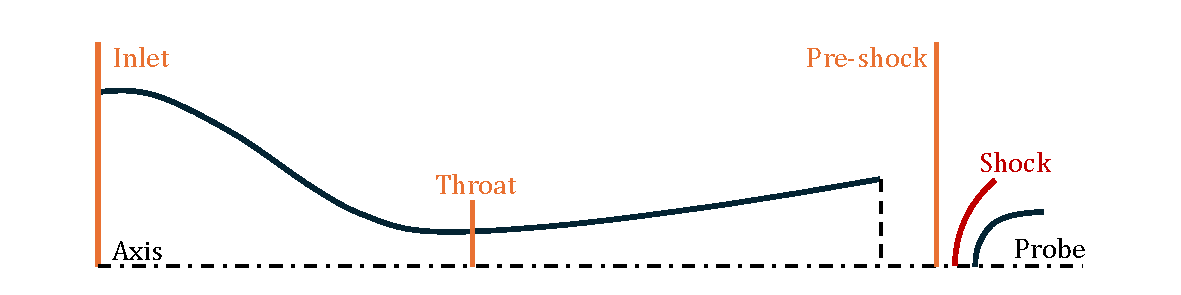
\includegraphics[width=0.9\textwidth,height=0.4\textheight,keepaspectratio]{../figures/cfd/LowFidelity.pdf}
        \end{column}
    \end{columns}
    \vspace{0.3cm}
    \textit{The fundamental discrepancy mimics the kind of severe, real-world model inadequacy that causes traditional calibration methods to fail.}
\end{frame}

\begin{frame}{Results: Reconstructing Catalytic Efficiencies}
    We calibrate the models using the KOH and Full Bayesian (FB) methods to rigorously evaluate the impact of these two model error types.
    
    \vspace{0.3cm}
    \begin{itemize}
        \item \textbf{Key Finding 1}: Ignoring model error (using standard Bayesian inversion) leads to severe bias and overconfidence; the inferred catalytic efficiencies absorb the un-modeled physics.
        \item \textbf{Key Finding 2}: Incorporating a proper model error term correctly inflates the uncertainty bounds, preventing dangerous false certitude in the design of thermal protection systems.
    \end{itemize}
\end{frame}
